% Compilar desde docs: latexmk -xelatex -interaction=nonstopmode -halt-on-error informe_final.tex
\documentclass[10pt,a4paper]{article}
\usepackage[margin=22mm,top=24mm,bottom=24mm,headheight=22pt]{geometry}
\usepackage{fontspec}
\setmainfont{texgyreheros}[Extension=.otf,UprightFont=*-regular,BoldFont=*-bold,ItalicFont=*-italic,BoldItalicFont=*-bolditalic]
\setsansfont{texgyreheros}[Extension=.otf,UprightFont=*-regular,BoldFont=*-bold,ItalicFont=*-italic,BoldItalicFont=*-bolditalic]
\setmonofont{texgyrecursor}[Scale=0.84,Extension=.otf,UprightFont=*-regular,BoldFont=*-bold,ItalicFont=*-italic,BoldItalicFont=*-bolditalic]
\usepackage[spanish,es-nodecimaldot,es-noshorthands]{babel}
\usepackage{microtype,graphicx,xcolor,booktabs,tabularx,array,longtable}
\usepackage{tikz}
\usetikzlibrary{positioning,arrows.meta,calc,backgrounds}
\usepackage[most]{tcolorbox}
\usepackage{titlesec,fancyhdr,enumitem,caption,subcaption,pdflscape,listings,float}
\usepackage{amsmath,amssymb}
\usepackage{hyperref,bookmark,xurl}
\definecolor{Slate}{HTML}{373946}
\definecolor{Wine}{HTML}{852A3B}
\definecolor{Sand}{HTML}{DEC1AF}
\definecolor{Plum}{HTML}{6C4B68}
\definecolor{Ink}{HTML}{20232D}
\definecolor{Muted}{HTML}{626574}
\definecolor{Paper}{HTML}{F6F3F0}
\definecolor{Line}{HTML}{DFE1E7}
\definecolor{Teal}{HTML}{24796C}
\hypersetup{hypertexnames=false,colorlinks=true,linkcolor=Wine,urlcolor=Plum,citecolor=Wine,pdftitle={Mining System — Informe final del proyecto},pdfauthor={Franco Parra},pdfsubject={Internet de las Cosas: nodo IoT, MySQL, API propia, Python y monitoreo en tiempo real}}
\urlstyle{same}
\renewcommand{\familydefault}{\sfdefault}
\setlength{\parindent}{0pt}
\setlength{\parskip}{5pt}
\linespread{1.1}
\setcounter{tocdepth}{1}
\AtBeginDocument{\spanishlcroman}
\widowpenalty=5000
\clubpenalty=5000
\setlength{\emergencystretch}{2em}
\setlist[itemize]{leftmargin=*,itemsep=3pt,topsep=4pt}
\setlist[enumerate]{leftmargin=*,itemsep=3pt,topsep=4pt}
\renewcommand{\arraystretch}{1.22}
\newcolumntype{Y}{>{\raggedright\arraybackslash}X}
\newcolumntype{P}[1]{>{\raggedright\arraybackslash}p{#1}}
\titleformat{\section}{\Large\bfseries\color{Slate}}{\textcolor{Wine}{\thesection}}{.7em}{}
\titleformat{\subsection}{\normalsize\bfseries\color{Wine}}{\thesubsection}{.6em}{}
\titlespacing*{\section}{0pt}{16pt}{10pt}
\titlespacing*{\subsection}{0pt}{12pt}{5pt}
\captionsetup{font=small,labelfont={bf,color=Wine},textfont={color=Muted},justification=raggedright,singlelinecheck=false,hypcap=false,skip=7pt}
\pagestyle{fancy}
\fancyhf{}
\fancyhead[L]{\scriptsize\bfseries\textcolor{Slate}{MINING SYSTEM}\quad\textcolor{Muted}{MEMORIA TÉCNICA}}
\fancyhead[R]{\scriptsize\textcolor{Muted}{INTERNET DE LAS COSAS · UCB}}
\fancyfoot[L]{\scriptsize\textcolor{Muted}{Franco Parra\quad /\quad 2026}}
\fancyfoot[R]{\textcolor{Wine}{\bfseries\thepage}}
\renewcommand{\headrulewidth}{.4pt}
\renewcommand{\headrule}{\hbox to\headwidth{\color{Line}\leaders\hrule height \headrulewidth\hfill}}
\newtcolorbox{insight}[1]{enhanced,breakable,colback=Paper,colframe=Paper,boxrule=0pt,borderline west={3pt}{0pt}{Wine},arc=3pt,left=11pt,right=11pt,top=8pt,bottom=8pt,title={#1},coltitle=Wine,fonttitle=\bfseries,attach title to upper={\par\smallskip},before skip=10pt,after skip=10pt}
\newcommand{\code}[1]{{\small\urlstyle{tt}\nolinkurl{#1}}}
\newcommand{\evidence}[2]{\textcolor{Wine}{\bfseries #1}\enspace\textcolor{Muted}{#2}}
\newcommand{\newsection}[1]{\clearpage\section{#1}}
\lstdefinestyle{project}{basicstyle=\ttfamily\scriptsize,backgroundcolor=\color{Paper},frame=single,framerule=.4pt,rulecolor=\color{Line},breaklines=true,breakatwhitespace=false,columns=fullflexible,keepspaces=true,showstringspaces=false,tabsize=2,aboveskip=9pt,belowskip=9pt,xleftmargin=5pt,xrightmargin=5pt,framexleftmargin=5pt,framexrightmargin=5pt,keywordstyle=\color{Wine}\bfseries,commentstyle=\color{Muted},stringstyle=\color{Teal},literate={á}{{\'a}}1 {é}{{\'e}}1 {í}{{\'i}}1 {ó}{{\'o}}1 {ú}{{\'u}}1 {ñ}{{\~n}}1 {Á}{{\'A}}1 {É}{{\'E}}1 {Ó}{{\'O}}1 {→}{{$\rightarrow$}}1}
\lstset{style=project}
\lstdefinelanguage{JSON}{morestring=[b]",morekeywords={true,false,null},sensitive=true}
\newcommand{\LatenciaLocal}{19{,}797}


\begin{document}
\begin{titlepage}
\thispagestyle{empty}
\begin{tikzpicture}[remember picture,overlay]
\fill[Slate] (current page.south west) rectangle (current page.north east);
\fill[Wine] ([xshift=18mm]current page.south west) rectangle ([xshift=23mm]current page.north west);
\fill[Sand] ([yshift=-23mm]current page.north west) rectangle ([xshift=80mm,yshift=-24mm]current page.north west);
\draw[white,opacity=.12,line width=.8pt] ([xshift=28mm,yshift=45mm]current page.south west)--++(35mm,42mm)--++(28mm,-27mm)--++(34mm,63mm)--++(55mm,-78mm);
\draw[white,opacity=.12] ([xshift=63mm,yshift=87mm]current page.south west)--++(7mm,-28mm)--++(21mm,1mm);
\draw[white,opacity=.12] ([xshift=125mm,yshift=123mm]current page.south west)--++(-9mm,-45mm)--++(20mm,13mm)--++(17mm,-46mm);
\foreach \x/\y in {37/43,66/69,104/48,145/78,170/44}{\fill[Sand,opacity=.7] ([xshift=\x mm,yshift=\y mm]current page.south west) circle(1.3mm);}
\draw[Sand,opacity=.35] ([xshift=37mm,yshift=43mm]current page.south west)--([xshift=66mm,yshift=69mm]current page.south west)--([xshift=104mm,yshift=48mm]current page.south west)--([xshift=145mm,yshift=78mm]current page.south west)--([xshift=170mm,yshift=44mm]current page.south west);
\end{tikzpicture}
\color{white}\hspace*{10mm}\begin{minipage}[t][.90\textheight][t]{.88\textwidth}
\vspace*{14mm}
{\small\bfseries UNIVERSIDAD CATÓLICA BOLIVIANA}\par
{\small Internet de las Cosas · Proyecto final}\par
\vspace{34mm}
{\fontsize{49}{51}\selectfont\bfseries MINING\\SYSTEM}\par
\vspace{7mm}
{\LARGE Manilla inteligente\\para mineros}\par
\vspace{8mm}
{\large\color{Sand} Comunicación, trazabilidad y monitoreo\\con infraestructura propia}\par
\vspace{15mm}
{\small\bfseries INFORME FINAL · DISEÑO Y VALIDACIÓN}\par
\vspace{4mm}
{\small Raspberry Pi\enspace /\enspace Python\enspace /\enspace API REST}\par
{\small MySQL\enspace /\enspace React\enspace /\enspace WebSocket}\par
\vfill
{\large\bfseries Franco Parra}\par
{\small La Paz, Bolivia · 14 de octubre de 2026}\par
\vspace{12mm}
\end{minipage}
\end{titlepage}
\pagenumbering{roman}
\section*{Resumen ejecutivo}
Mining System integra una manilla basada en Raspberry Pi Zero 2 W con una central de operaciones alojable en Raspberry Pi 4. Su propósito es que un trabajador pueda emitir reportes predeterminados desde una pantalla OLED y tres pulsadores, y que el personal autorizado reciba esos eventos con identidad, zona y fecha en una interfaz centralizada.

La solución utiliza software e infraestructura propios: Python en el nodo, ASP.NET Core 10 en el servidor, MySQL para persistencia y React 19 con TypeScript para la interfaz. La API REST administra usuarios, dispositivos e historial; el envío de eventos desde la manilla utiliza WebSocket y la actualización de la web emplea SignalR sobre WebSocket. Una cola local de archivos JSON conserva los reportes cuando se interrumpe la red y solo los elimina después de recibir una confirmación de persistencia.

El trabajo documenta el circuito completo, el modelo relacional, los contratos de comunicación, la autenticación por roles, el programa del nodo, el dashboard y el despliegue. La validación ejecutada comprende \textbf{40 pruebas automatizadas satisfactorias}: 16 de la manilla, 16 de integración API/MySQL y 8 de navegador. Se añaden evidencias de solicitudes HTTP reales, inserción y lectura en MySQL, entrega de eventos y capturas de la aplicación.

El circuito incorpora además SEN0564, ADS1115, MLX90614, INMP441, buzzer, LED RGB y motor vibrador. Sus conexiones están definidas, pero la integración y calibración de sus controladores físicos se mantienen como alcance pendiente. Las lecturas utilizadas en las pruebas son datos controlados; no constituyen mediciones obtenidas en una mina.

\begin{insight}{Alcance y fidelidad técnica}
Esta memoria describe la implementación existente y su migración verificada a MySQL. El nodo ejecuta \textbf{CPython sobre Linux}, y la visualización está construida en \textbf{React}; no se atribuye al proyecto el uso de MicroPython, un dashboard desarrollado en Python ni Supabase. Las evidencias de software se distinguen del montaje y de la validación física pendientes.
\end{insight}
\vspace{3mm}
\textbf{Palabras clave:} nodo IoT, Raspberry Pi, MySQL, API REST, Python, comunicación en tiempo real, control de acceso, trazabilidad.

\clearpage\tableofcontents
\clearpage\pagenumbering{arabic}

\section{Contexto, objetivos y alcance}
\label{sec:contexto}
\subsection{Problema que aborda el proyecto}
La supervisión de un equipo distribuido requiere identificar quién emite un reporte, desde qué zona y en qué momento se recibe. Un registro aislado o un mensaje sin vínculo con su portador dificulta el seguimiento de incidentes y la reconstrucción de la jornada. El proyecto concentra esa información en una central y simplifica la interacción del trabajador mediante un catálogo acotado de mensajes.

La manilla es un \textbf{prototipo académico de comunicación y monitoreo}. Su validación actual demuestra el recorrido de mensajes entre nodo, persistencia y operador; no demuestra cobertura de radio dentro de una mina ni certificación de un equipo de protección.

\subsection{Objetivo general}
Diseñar e implementar una plataforma IoT propia que vincule un nodo portátil con una central de operaciones, permita reportes identificados y persistentes, y presente la información a usuarios autorizados mediante una interfaz actualizada por eventos.

\subsection{Objetivos específicos}
\begin{enumerate}
\item Definir las conexiones del nodo, sus buses, alimentación e interfaz de usuario.
\item Organizar usuarios, manillas, mensajes, lecturas y auditoría en un modelo relacional MySQL.
\item Desarrollar una API REST para la administración y consulta, complementada con WebSocket para eventos de campo.
\item Implementar en Python navegación, confirmación de envío, almacenamiento local y reconexión.
\item Proteger el acceso mediante autenticación, roles, credenciales de dispositivo e invalidación de sesiones.
\item Visualizar presencia, mensajes y lecturas con recuperación después de una interrupción.
\item Verificar el funcionamiento con pruebas reproducibles y adjuntar sus evidencias.
\end{enumerate}

\subsection{Actores y flujo funcional}
El \textbf{administrador} crea cuentas y mantiene la configuración; el \textbf{supervisor} consulta la operación, administra manillas y revisa alertas; el \textbf{minero} es el portador asignado al nodo y reporta desde la OLED. Las cuentas de minero no acceden al panel de operaciones.

El flujo implementado es \emph{manilla $\rightarrow$ central $\rightarrow$ operador}. Marcar una alerta como revisada añade autor y fecha al historial central. Esa acción no transmite una respuesta al trabajador ni declara resuelto el incidente.

\newsection{Arquitectura de la solución}
\label{sec:arquitectura}
\subsection{Separación de responsabilidades}
El nodo reúne interacción y transporte; la API valida reglas de negocio y acceso; MySQL conserva los registros; la web presenta el estado operativo. Esta separación permite evolucionar la interfaz o los sensores sin mezclar la lectura de GPIO con la administración de cuentas.

\begin{figure}[ht]
\centering
\begin{tikzpicture}[node distance=11mm and 13mm,box/.style={draw=Line,rounded corners=4pt,fill=Paper,minimum width=4.6cm,minimum height=1.35cm,align=center,font=\small},arrow/.style={-{Latex[length=2.5mm]},thick,draw=Wine}]
\node[box] (node) {\textbf{Nodo IoT · Zero 2 W}\\Python · OLED · botones\\Cola JSON persistente};
\node[box,right=of node] (api) {\textbf{Central · ASP.NET Core}\\API REST · ingestión\\Autenticación · SignalR};
\node[box,below=of api] (db) {\textbf{MySQL}\\Usuarios · manillas · mensajes\\Lecturas · auditoría};
\node[box,below=of node] (web) {\textbf{Operador · React}\\Dashboard · alertas\\Historial · administración};
\draw[arrow] (node) -- node[above,font=\scriptsize]{WebSocket / Wi-Fi} (api);
\draw[arrow,<->] (api) -- node[right,font=\scriptsize]{EF Core} (db);
\draw[arrow] (api.south west) -- node[above,sloped,font=\scriptsize]{SignalR: eventos} (web.north east);
\draw[arrow] (web.west) -- ++(-8mm,0) |- node[pos=.73,above,font=\scriptsize]{REST: gestión y consulta} ([yshift=8mm]api.north) -- (api.north);
\end{tikzpicture}
\caption{Arquitectura lógica del sistema implementado. La Pi 4 puede alojar la central; su enlace con la manilla es de red, sin unión de sus GPIO.}
\label{fig:arquitectura}
\end{figure}

\subsection{Tecnologías y decisiones}
\begin{tabularx}{\linewidth}{@{}P{31mm}P{45mm}Y@{}}
\toprule\textbf{Capa} & \textbf{Tecnología} & \textbf{Responsabilidad}\\\midrule
Nodo & Python, gpiozero, Pillow, luma.oled & Entrada por botones, dibujo OLED y transporte con cola local.\\
Servidor & ASP.NET Core 10, EF Core & Contratos, validaciones, roles e ingestión de eventos.\\
Persistencia & MySQL, migraciones EF & Datos relacionales, índices, claves foráneas y transacciones.\\
Interfaz & React 19, TypeScript & Panel de operación, formularios, gráficos y adaptación móvil.\\
Tiempo real & WebSocket, SignalR & Envío del nodo y notificación inmediata al navegador.\\
Despliegue & Docker Compose, Nginx & Servicios aislados, proxy de origen único y volúmenes persistentes.\\\bottomrule
\end{tabularx}

MySQL funciona como un servicio independiente de la API. Su selección facilita separar la administración del almacenamiento, mantener un esquema versionado y utilizar respaldos lógicos. El cambio de motor no implica por sí mismo escalabilidad ilimitada: la configuración actual mantiene una instancia central y sus reglas de exclusión de mutaciones.

\subsection{Red y comportamiento sin conexión}
La Zero 2 W incorpora Wi-Fi de 2,4 GHz y un procesador de cuatro núcleos con 512 MB de memoria\cite{rpi}. La central y el nodo requieren una ruta de red disponible. Cuando esa ruta falla, la manilla conserva los mensajes y reintenta el enlace; la recepción inmediata solo es posible durante la conectividad efectiva.

\newsection{Diseño del nodo IoT y del circuito}
\label{sec:circuito}
\subsection{Componentes e interfaces}
La Raspberry Pi Zero 2 W actúa como nodo de campo. El diseño usa la cabecera de 40 pines, GPIO de 3,3 V y dos buses independientes: I\textsuperscript{2}C para pantalla y sensores, e I\textsuperscript{2}S para el micrófono. La Pi no dispone de entradas analógicas integradas; el ADS1115 permite incorporar la salida del SEN0564.

\begin{tabularx}{\linewidth}{@{}P{30mm}P{36mm}Y@{}}
\toprule\textbf{Componente} & \textbf{Interfaz} & \textbf{Función y estado}\\\midrule
OLED SSD1306 & I\textsuperscript{2}C, \code{0x3C} & Menú de 128\,$\times$\,64 y confirmación de reportes implementados.\\
Tres pulsadores & GPIO17, 27 y 22 & Subir, bajar y confirmar; pull-up interno y filtrado de rebote.\\
ADS1115 & I\textsuperscript{2}C, \code{0x48} & ADC de 16 bits; A0 recibe la señal de CO. Integración física pendiente.\\
SEN0564 & Salida analógica A & Sensor cualitativo de CO; requiere calibración antes de expresar ppm\cite{co}.\\
MLX90614 & I\textsuperscript{2}C, \code{0x5A} & Medición infrarroja. Se especifica una variante compatible con 3,3 V.\\
INMP441 & I\textsuperscript{2}S & Audio digital; conexiones definidas, captura aún no integrada.\\
Buzzer y LED RGB & GPIO24; GPIO5/6/13 & Alertas acústicas y visuales previstas en el cableado.\\
Motor vibrador & GPIO23 + NPN & Alerta háptica mediante etapa de potencia y protección inductiva.\\\bottomrule
\end{tabularx}

\subsection{Distribución eléctrica}
La Pi se alimenta mediante su entrada micro-USB de 5 V. Los módulos toman \textbf{3,3 V del pin físico 1} y comparten \textbf{GND desde el pin 6}. Los pines físicos 2 y 4 de 5 V no se conectan a los módulos. La central tiene alimentación propia y no se une por cable al GPIO de la manilla.

SDA y SCL se conectan en paralelo a la OLED, el ADS1115 y el MLX90614. Sus direcciones distintas evitan conflictos de selección. ADDR del ADS1115 se fija a GND; ALRT y A1--A3 quedan libres. El SEN0564 se alimenta a 3,3 V y entrega su salida A directamente a A0.

Los pulsadores cierran hacia tierra y no necesitan una línea VCC. En un pulsador de cuatro patas se debe seleccionar un contacto de cada grupo interno; unir dos patas ya conectadas no genera la transición esperada.

\begin{insight}{Qué valida el diagrama}
El proyecto Wokwi contiene 51 conexiones y pasa \code{wokwi-cli lint --warnings-as-errors}. La ilustración permite revisar terminales y recorrido de cables. Esta validación estructural no simula Raspberry Pi OS ni certifica el funcionamiento eléctrico de los sensores.
\end{insight}

\clearpage
\subsection{Mapa de conexiones}
Los números BCM utilizados por Python y los números físicos de la cabecera son distintos. La tabla mantiene ambas referencias para evitar errores de montaje.

\begin{tabularx}{\linewidth}{@{}P{34mm}P{28mm}P{28mm}Y@{}}
\toprule\textbf{Señal} & \textbf{GPIO BCM} & \textbf{Pin físico} & \textbf{Destino}\\\midrule
Alimentación & -- & 1 / 6 & Línea común de 3,3 V / GND.\\
SDA / SCL & 2 / 3 & 3 / 5 & OLED, ADS1115 y MLX90614.\\
Subir / bajar / Enter & 17 / 27 / 22 & 11 / 13 / 15 & Pulsadores hacia GND.\\
SCK / WS / SD & 18 / 19 / 20 & 12 / 35 / 38 & INMP441; L/R a GND.\\
Motor & 23 & 16 & Resistencia de 1 k$\Omega$ a la base del NPN.\\
Buzzer & 24 & 18 & Terminal I/O del módulo de tres pines.\\
LED rojo / verde / azul & 5 / 6 / 13 & 29 / 31 / 33 & Canales del LED RGB.\\
Reservados para audio & 16 / 21 & 36 / 40 & Sin conexiones adicionales.\\\bottomrule
\end{tabularx}

\subsection{Protección del motor y variantes de módulos}
El motor de dos cables no se acciona directamente desde el GPIO. Su positivo va a 3,3 V y su negativo al colector del NPN; el emisor va a GND. GPIO23 llega a la base mediante 1 k$\Omega$, y una resistencia de 10 k$\Omega$ entre base y tierra mantiene la salida apagada durante el arranque. El diodo de rueda libre y el condensador de 100 nF se conectan en paralelo con el motor. El cátodo del diodo va a 3,3 V y el ánodo al colector.

El orden físico de B, C y E se identifica con la hoja de datos del transistor concreto. El dibujo lógico no sustituye esa comprobación. En el LED RGB se representa cátodo común y resistencias de 220 $\Omega$ en rojo y 100 $\Omega$ en verde y azul; si el módulo incorpora sus resistencias, se omiten las externas. La polaridad de activación del buzzer depende de la variante de módulo y debe verificarse en banco.

\subsection{Lectura analógica y calibración}
La conversión de una cuenta firmada del ADS1115 a tensión depende del rango programado. Para un rango de $\pm4{,}096$ V se obtiene:
\[
V_{A0}=\frac{N}{32768}\,4{,}096\ \mathrm{V}.
\]
Esta expresión calcula \textbf{voltios}, no concentración de CO. El campo \code{gasPpm} solo debe poblarse con una conversión calibrada. El proyecto no define umbrales de seguridad a partir de una lectura cualitativa y no representa la temperatura IR de objeto como temperatura corporal.

\subsection{Montaje por etapas}
La puesta en marcha se organiza en OLED y botones; bus I\textsuperscript{2}C y entrada analógica; micrófono I\textsuperscript{2}S; y salidas de alerta. El documento \code{docs/conexiones.tex} contiene las pruebas de cada grupo. Una estimación de consumo o autonomía requiere mediciones del conjunto real; no se presenta como resultado experimental en esta memoria.

\clearpage
\section*{Plano de montaje del nodo}
\begin{figure}[ht]
\centering
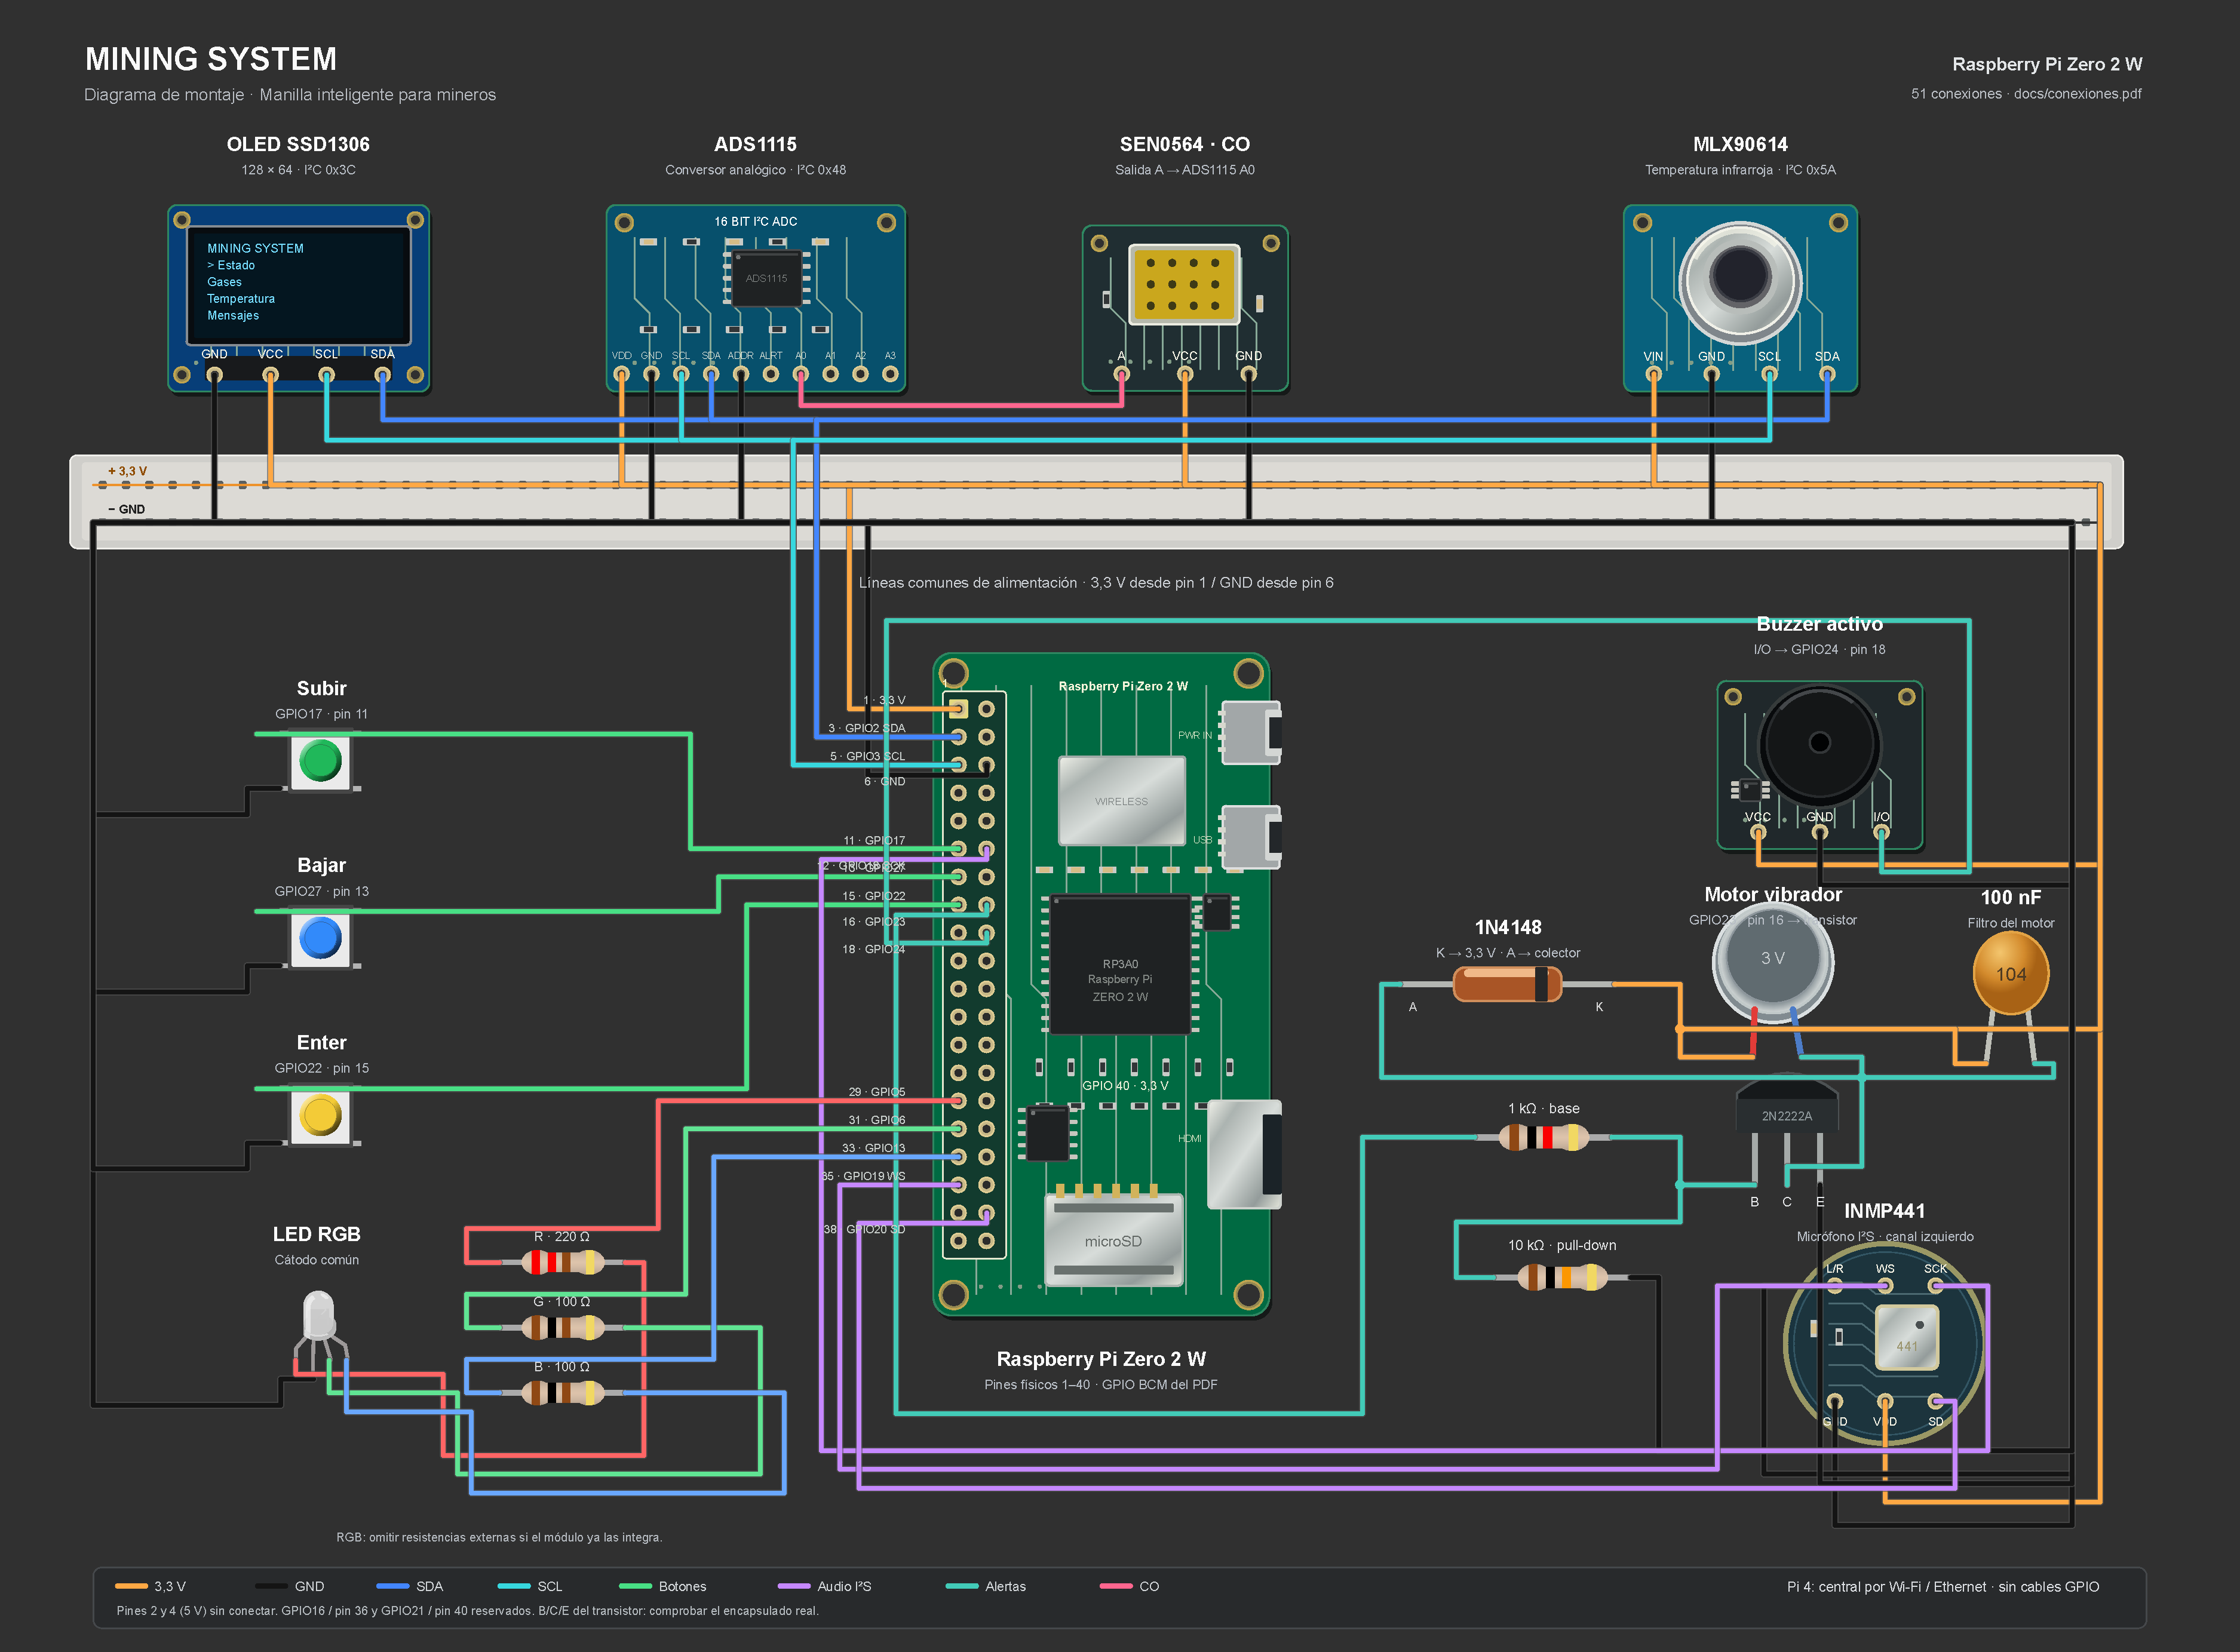
\includegraphics[width=\linewidth]{informe/figuras/circuito.pdf}
\caption{Diagrama ilustrado del proyecto, con componentes y 51 conexiones tomadas del archivo Wokwi. Es una representación de montaje, no una fotografía ni evidencia de medición física. Los pulsadores, resistencias y LED usan dibujos de Wokwi Elements; los demás módulos son ilustraciones propias.}
\label{fig:circuito}
\end{figure}
\subsection*{Lectura del plano}
El color naranja identifica la alimentación de 3,3 V y el negro la tierra común. Azul y turquesa corresponden a SDA y SCL; verde, a los botones; violeta, al micrófono I\textsuperscript{2}S. Los cables de los canales rojo, verde y azul permiten seguir cada rama del LED. La etapa del motor incorpora el NPN, el diodo, el condensador y ambas resistencias.

El archivo vectorial adjunto permite ampliar el dibujo sin perder definición. Las correspondencias exactas entre BCM y pin físico se consultan en la tabla de conexiones; el archivo \code{docs/wokwi/diagram.json} conserva los terminales de cada cable para su edición y validación.

\newsection{Modelo de datos y persistencia MySQL}
\label{sec:datos}
\subsection{Entidades y significado}
El modelo almacena cinco entidades de dominio. Los usuarios y las manillas utilizan identificadores de 32 caracteres; los mensajes, lecturas y eventos poseen claves numéricas autoincrementales. Las relaciones se materializan mediante claves foráneas de MySQL.

\begin{tabularx}{\linewidth}{@{}P{25mm}P{30mm}Y@{}}
\toprule\textbf{Tabla} & \textbf{Clave / relación} & \textbf{Contenido y finalidad}\\\midrule
\code{Users} & \code{Id}; correo único & Identidad, rol, estado, hash de contraseña y versión de sesión.\\
\code{Devices} & \code{Id}; \code{UserId} & Nombre, zona, hash de credencial, activación y última presencia.\\
\code{Messages} & \code{Id}; \code{DeviceId} & Reporte, identificador de origen, identidad histórica y revisión.\\
\code{Readings} & \code{Id}; \code{DeviceId} & Temperatura, CO calibrado, batería y fecha de recepción.\\
\code{Events} & \code{Id} & Actor, descripción y fecha de acciones administrativas.\\\bottomrule
\end{tabularx}

Un usuario puede tener varias asignaciones históricas de manillas; la regla de aplicación permite una sola manilla activa por minero. Una manilla puede existir sin asignación, pero necesita un minero activo para enviar mensajes. Cada dispositivo se relaciona con muchos mensajes y muchas lecturas. La auditoría conserva el nombre del actor como texto y no establece una clave foránea a usuarios.

\subsection{Integridad, índices y trazabilidad}
El correo, el nombre de manilla y el hash de su credencial poseen índices únicos. La combinación \code{(DeviceId, ClientMessageId)} también es única: implementa la protección persistente frente a reintentos del mismo reporte. Se añaden índices por recepción de mensajes y por dispositivo/fecha de lecturas.

\code{MinerName}, \code{DeviceName} y \code{Zone} se copian al mensaje en el momento de recibirlo. Esta duplicación deliberada evita que una reasignación cambie el significado del historial. La identidad del revisor también se conserva como texto. Desactivar una cuenta o dispositivo no elimina sus registros anteriores.

Las fechas se normalizan a UTC y se guardan como \code{datetime(6)}. Como ese tipo no contiene la zona horaria, un conversor de EF Core restablece explícitamente UTC al leer. La interfaz presenta las fechas en \code{America/La_Paz}. Las mediciones ausentes se almacenan como \code{NULL}; ausencia y valor cero no significan lo mismo.

\subsection{Migración aplicada}
La migración inicial de EF Core crea tablas, claves e índices; el historial técnico de migraciones constituye una sexta tabla del motor. La configuración local y Docker usan MySQL. Se retiraron los proveedores SQLite del backend y el almacenamiento SQLite del nodo.

El archivo anterior se exportó en solo lectura y se importó en una transacción sobre una base vacía, conservando \textbf{un usuario y un evento de auditoría}. El archivo original permaneció intacto. La importación rechaza una base que ya tenga datos y no imprime hashes ni contraseñas. El esquema SQL completo se adjunta en \code{informe/evidencias/mysql-schema.sql}.

\clearpage
\subsection{Diagrama entidad--relación}
\begin{figure}[ht]
\centering
\resizebox{\linewidth}{!}{\begin{tikzpicture}[entity/.style={draw=Line,rounded corners=3pt,fill=Paper,align=left,text width=4.6cm,inner sep=9pt,font=\small},rel/.style={thick,draw=Wine}]
\node[entity] (u) at (0,0) {\textcolor{Wine}{\textbf{Users}}\\\rule{4.5cm}{.4pt}\\\textbf{PK} Id: varchar(32)\\Name: varchar(100)\\Email: varchar(180) \textbf{UQ}\\Role: varchar(16)\\Active: bool\\PasswordHash: varchar(512)\\SessionVersion: varchar(32)\\CreatedAt: datetime(6)};
\node[entity] (d) at (6.7,0) {\textcolor{Wine}{\textbf{Devices}}\\\rule{4.5cm}{.4pt}\\\textbf{PK} Id: varchar(32)\\Name: varchar(60) \textbf{UQ}\\Zone: varchar(100)\\\textbf{FK} UserId: varchar(32), NULL\\KeyHash: varchar(64) \textbf{UQ}\\Active: bool\\LastSeenAt: datetime(6), NULL\\CreatedAt: datetime(6)};
\node[entity] (m) at (0,-6.2) {\textcolor{Wine}{\textbf{Messages}}\\\rule{4.5cm}{.4pt}\\\textbf{PK} Id: bigint, AI\\\textbf{FK} DeviceId: varchar(32)\\ClientMessageId: varchar(80)\\Code: varchar(16)\\MinerName: varchar(100)\\DeviceName: varchar(60)\\Zone: varchar(100)\\SentAt / ReceivedAt: datetime(6)\\ReviewedAt: datetime(6), NULL\\ReviewedBy: varchar(100), NULL\\\textbf{UQ} (DeviceId, ClientMessageId)};
\node[entity] (r) at (6.7,-6.2) {\textcolor{Wine}{\textbf{Readings}}\\\rule{4.5cm}{.4pt}\\\textbf{PK} Id: bigint, AI\\\textbf{FK} DeviceId: varchar(32)\\TemperatureC: double, NULL\\GasPpm: double, NULL\\BatteryPercent: double, NULL\\ReceivedAt: datetime(6)};
\node[entity] (e) at (13.4,-3.1) {\textcolor{Wine}{\textbf{Events}}\\\rule{4.5cm}{.4pt}\\\textbf{PK} Id: bigint, AI\\Actor: varchar(100)\\Description: varchar(500)\\CreatedAt: datetime(6)\\\medskip\textcolor{Muted}{Auditoría sin FK al actor.}};
\draw[rel] (u.east)--node[above,font=\small]{0..1\quad: \quad N}(d.west);
\draw[rel] (d.south)--node[right,font=\small]{1 : N}(r.north);
\draw[rel] (d.south west)--++(-.4,-.5)-|node[pos=.75,left,font=\small]{1 : N}(m.north);
\end{tikzpicture}}
\caption{Modelo correspondiente a las entidades, el mapeo EF Core y las claves foráneas comprobadas en MySQL. AI: autoincremento; UQ: restricción única. La regla de una manilla activa por minero se valida en la API.}
\label{fig:er}
\end{figure}

\begin{insight}{Evidencia de relaciones reales}
La consulta a \code{information_schema.KEY_COLUMN_USAGE} identificó \code{Devices.UserId → Users.Id}, \code{Messages.DeviceId → Devices.Id} y \code{Readings.DeviceId → Devices.Id}. Su resultado se conserva en \code{informe/evidencias/api-mysql.json}.
\end{insight}

\newsection{API propia, inserción y lectura de información}
\label{sec:api}
\subsection{Dos canales con funciones distintas}
La API REST propia atiende la gestión y las consultas del panel. El dispositivo transmite mensajes y telemetría por \textbf{WebSocket nativo} a \code{/ws/device}. El servidor persiste esos eventos en MySQL y los publica hacia la web mediante SignalR. Por tanto, el proyecto integra HTTP y eventos persistentes sin utilizar Supabase ni una API externa de almacenamiento.

\begin{tabularx}{\linewidth}{@{}P{16mm}P{65mm}Y@{}}
\toprule\textbf{Método} & \textbf{Ruta} & \textbf{Finalidad}\\\midrule
POST & \code{/api/auth/setup} & Crear al primer administrador.\\
POST & \code{/api/auth/login} & Verificar acceso y emitir cookie.\\
POST / PUT & \code{/api/users} / \code{/api/users/{id}} & Registrar o actualizar usuarios.\\
POST / PUT & \code{/api/devices} / \code{/api/devices/{id}} & Registrar, asignar o editar manillas.\\
GET & \code{/api/overview} & Contadores y últimos mensajes.\\
GET & \code{/api/messages} & Historial paginado y filtrable.\\
GET & \code{/api/devices/{id}/telemetry} & Últimas 100 lecturas del dispositivo.\\
POST & \code{/api/messages/{id}/review} & Revisión interna de una alerta crítica.\\
GET & \code{/api/events} & Últimas 100 acciones administrativas.\\\bottomrule
\end{tabularx}

Las solicitudes usan JSON y las mutaciones web requieren \code{X-Mining-Client: web}. El servidor aplica validaciones de longitud, correo, roles, rango de lecturas y estado de asignación. Los perfiles y dispositivos devueltos excluyen hashes de contraseña y de credenciales. El contrato de desarrollo está disponible en \code{/openapi/v1.json}.

\subsection{Inserción mediante WebSocket}
El nodo conecta con la cabecera \code{X-Device-Key}. El servidor valida su hash al conectar y al procesar cada trama. Para un mensaje verifica catálogo, asignación e identificador estable; para telemetría exige al menos una medición y valida sus rangos de transporte. Después ejecuta \code{SaveChangesAsync()}, emite el evento en vivo y devuelve un \code{ack}.

\begin{lstlisting}[language=Python,caption={Orden esencial de recepción y confirmación, extraído de la lógica del servidor.}]
# Secuencia de DeviceIngestion.Process (servidor ASP.NET Core):
autenticar_credencial_y_dispositivo()
validar_trama_y_reglas_de_negocio()
buscar_por_deviceId_y_clientMessageId()
guardar_en_MySQL()
publicar_evento_SignalR_si_es_nuevo()
devolver_ack_con_el_id_persistido()
\end{lstlisting}
El listado anterior expresa el flujo en pseudocódigo; la implementación real está en \code{backend/Services/DeviceIngestion.cs}. No es un endpoint REST alternativo ni un script que se ejecute en la manilla.

\clearpage
\subsection{Prueba reproducible de un reporte}
La evidencia E-API creó una base MySQL temporal, registró cuentas de prueba y una manilla, y envió la siguiente trama. El servidor devolvió la confirmación y el navegador suscrito recibió \code{MessageReceived}.

\lstinputlisting[language=JSON,caption={Trama realmente enviada en la prueba E-API.}]{informe/evidencias/trama.json}
\lstinputlisting[language=JSON,caption={Confirmación real, recibida después de persistir el reporte.}]{informe/evidencias/ack.json}

Reenviar la misma trama produjo \code{duplicate: true} y el mismo \code{messageId}. La consulta del historial devolvió un único mensaje. Se comprobó así que el reintento no aumenta la cantidad de reportes persistidos.

\subsection{Lectura y errores comprobados}
La misma sesión realizó \code{GET /api/messages} y \code{GET /api/devices/{id}/telemetry}. Se recuperaron un mensaje y una lectura controlada con temperatura de 28,6\,$^\circ$C, gas de 410 ppm y batería de 86\,\%. Esos valores fueron \textbf{inyectados por la prueba}: verifican el contrato de datos y la persistencia, no una medición ni calibración de sensores.

\begin{tabularx}{\linewidth}{@{}P{52mm}P{26mm}Y@{}}
\toprule\textbf{Situación ensayada} & \textbf{Respuesta} & \textbf{Resultado observado}\\\midrule
Consulta sin sesión & HTTP 401 & No entrega información protegida.\\
Contraseña incorrecta & HTTP 401 & No inicia sesión.\\
Correo duplicado & HTTP 409 & No crea una segunda cuenta.\\
Registro autorizado & HTTP 200 & Inserta y devuelve un perfil sin hash.\\
Batería en 101\,\% & Trama \code{error} & Rechaza una lectura fuera del contrato.\\
Reenvío del mismo mensaje & \code{ack}, duplicado & Conserva un único registro.\\\bottomrule
\end{tabularx}

Los límites admitidos por el transporte son de $-50$ a 150\,$^\circ$C, de 0 a 1\,000\,000 ppm y de 0 a 100\,\% de batería. Son límites de validación de datos y no umbrales de riesgo.

\newsection{Software Python del nodo y entrega persistente}
\label{sec:python}
\subsection{Entorno de ejecución y organización}
El nodo ejecuta \textbf{Python 3 sobre Raspberry Pi OS}. Se emplean \code{gpiozero} para botones, \code{luma.oled} para la pantalla, Pillow para generar fotogramas y \code{websockets} para el cliente de red. El simulador usa Tkinter y conserva el mismo estado de navegación y el mismo renderizador.

Esta elección corresponde a una computadora Linux con procesos, hilos y sistema de archivos. No se utiliza MicroPython ni se ejecuta este programa en una Raspberry Pi Pico. La distinción conserva coherencia entre el hardware del proyecto y las bibliotecas efectivamente implementadas.

\begin{tabularx}{\linewidth}{@{}P{58mm}Y@{}}
\toprule\textbf{Archivo} & \textbf{Responsabilidad}\\\midrule
\code{src/main.py} & Inicialización, modo hardware/simulador y liberación de recursos.\\
\code{src/config.py} & Configuración JSON, validación de GPIO y rutas.\\
\code{src/input/buttons.py} & Convertir pulsaciones en acciones encoladas.\\
\code{src/display/menu.py} & Máquina de estados de navegación y envío.\\
\code{src/display/renderer.py} & Generar imágenes monocromas de 128\,$\times$\,64.\\
\code{src/communication/client.py} & Cola JSON, WebSocket, reintentos y confirmaciones.\\\bottomrule
\end{tabularx}

\subsection{Interacción sin envíos accidentales}
Subir y bajar cambian la selección; Enter abre una opción. En Mensajes, seleccionar un reporte abre una segunda pantalla con Enviar y Cancelar. La trama solo se encola al confirmar Enviar. La interfaz distingue \emph{Sin configurar}, \emph{Guardado en cola}, \emph{Enviado a central} y \emph{Error al guardar}.

Los callbacks GPIO únicamente colocan acciones en una cola de trabajo. El hilo principal actualiza la pantalla, evitando dibujar desde callbacks concurrentes. Los pines reservados por I\textsuperscript{2}C e I\textsuperscript{2}S se rechazan durante la carga de configuración.

\begin{lstlisting}[language=Python,caption={Callbacks implementados para navegación con pull-up y rebote filtrado.}]
for name, action in (("up", Action.UP),
                     ("down", Action.DOWN),
                     ("enter", Action.ENTER)):
    button = Button(config[name], pull_up=True,
                    bounce_time=config["bounce_seconds"])
    button.when_pressed = lambda event=action: queue.put(event)
\end{lstlisting}

\clearpage
\subsection{Cola local de archivos y confirmación}
Cada mensaje conserva un UUID y una fecha UTC. Se escribe primero en un archivo temporal, se fuerza su contenido con \code{fsync}, se renombra de forma atómica y se sincroniza el directorio. Un bloqueo de archivo coordina a escritores concurrentes. La cola no depende de MySQL ni de disponibilidad de red para registrar el reporte.

\begin{lstlisting}[language=Python,caption={Secuencia real de vaciado de la cola, en DeviceClient.}]
queued = self.outbox.first()
if queued:
    message_id, payload = queued
    self._exchange(socket, payload)
    self.outbox.acknowledge(message_id)
    self.events.put(TransportEvent("delivered", message_id))
\end{lstlisting}
\code{_exchange()} exige una trama \code{ack} cuyo \code{clientMessageId} corresponda al mensaje y contenga un identificador central válido. Una confirmación ajena produce un error y mantiene el reporte pendiente. Si se pierde un \code{ack}, el mensaje vuelve a enviarse con su mismo UUID y la clave única de MySQL impide duplicarlo.

La reconexión usa esperas de 1, 2, 4, 8, 16 y hasta 20 segundos. El heartbeat se envía por defecto cada 20 segundos. El servidor cierra sockets inactivos y calcula presencia con una ventana de 90 segundos; esa presencia no sustituye una lectura de sensores.

\begin{figure}[ht]
\centering
\begin{subfigure}{.24\linewidth}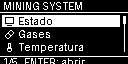
\includegraphics[width=\linewidth]{informe/figuras/oled-menu.png}\caption{Menú.}\end{subfigure}\hfill
\begin{subfigure}{.24\linewidth}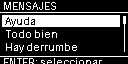
\includegraphics[width=\linewidth]{informe/figuras/oled-mensajes.png}\caption{Catálogo.}\end{subfigure}\hfill
\begin{subfigure}{.24\linewidth}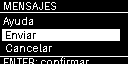
\includegraphics[width=\linewidth]{informe/figuras/oled-confirmacion.png}\caption{Confirmar.}\end{subfigure}\hfill
\begin{subfigure}{.24\linewidth}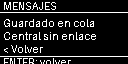
\includegraphics[width=\linewidth]{informe/figuras/oled-cola.png}\caption{En cola.}\end{subfigure}
\caption{Fotogramas generados por el renderizador real de la aplicación en una secuencia controlada. Son evidencia de la interfaz de software, no fotografías de una pantalla conectada.}
\label{fig:oled}
\end{figure}

\subsection{Punto de integración de telemetría}
\code{DeviceClient} admite un proveedor opcional \code{telemetry}. Si devuelve mediciones, el cliente transmite una trama de telemetría en lugar del heartbeat; si no hay proveedor, conserva el enlace sin inventar valores. En el arranque actual del nodo, los controladores de sensores no están conectados a ese proveedor. La interfaz conserva las lecturas físicas como pendientes.

\begin{insight}{Resultado verificado}
Las pruebas demuestran confirmación explícita antes de encolar, supervivencia de la cola al reiniciar, rechazo de ACK ajeno, preservación de 32 escrituras concurrentes y ausencia de mensajes cuando falla la escritura atómica. Un fallo de almacenamiento nunca se muestra como entrega exitosa.
\end{insight}

\newsection{Registro, autenticación y autorización}
\label{sec:auth}
\subsection{Alta inicial y gestión de cuentas}
Cuando no existen usuarios, \code{/api/auth/status} indica que se requiere configuración. La pantalla inicial permite crear al primer administrador; después, \code{/api/auth/setup} deja de admitir nuevas altas iniciales. Las demás cuentas se registran desde Usuarios por un administrador autenticado.

El servidor normaliza los correos, exige un nombre válido y aplica una contraseña de al menos 10 caracteres al crear o cambiar credenciales. No hay contraseñas predeterminadas. \code{PasswordHasher<User>} genera y verifica el hash; el texto original no se almacena en las tablas ni se entrega al frontend\cite{cookie}.

\begin{tabularx}{\linewidth}{@{}P{28mm}YYY@{}}
\toprule\textbf{Operación} & \textbf{Admin} & \textbf{Supervisor} & \textbf{Minero}\\\midrule
Consultar central & Sí & Sí & No\\
Mensajes y revisión & Sí & Sí & Desde el nodo\\
Gestionar manillas & Sí & Sí & No\\
Gestionar usuarios & Sí & No & No\\
Cambiar contraseña propia & Sí & Sí & Sin acceso al panel\\\bottomrule
\end{tabularx}

Se impide desactivar la propia cuenta y eliminar al último administrador activo. Antes de desactivar a un minero o modificar su rol deben desasignarse sus manillas activas. La autorización se verifica en el servidor; ocultar un botón no constituye el mecanismo de protección.

\subsection{Sesiones y protección de solicitudes}
La sesión utiliza la cookie \code{mining.session}, con \code{HttpOnly}, \code{SameSite=Strict} y duración de ocho horas, sin renovación deslizante. En HTTPS se marca Secure. El frontend no guarda tokens en \code{localStorage}. Las mutaciones requieren el encabezado propio del cliente y se rechazan orígenes no autorizados.

Cada usuario posee \code{SessionVersion}. Cambiar contraseña, permisos o estado invalida sesiones anteriores; las conexiones en vivo también se revocan. El inicio de sesión y la configuración inicial tienen un límite de 12 solicitudes por IP por minuto. Las claves de protección de cookies se guardan fuera de las imágenes de despliegue.

\subsection{Credenciales independientes para la manilla}
Registrar una manilla genera una credencial aleatoria de 64 caracteres, visible una sola vez. La central guarda su hash SHA-256 y recibe el valor original en \code{X-Device-Key}; no se incluye en una URL. La rotación invalida la credencial anterior y corta su uso en sockets activos.

\clearpage
\subsection{Evidencias de la experiencia de acceso y registro}
\begin{figure}[H]
\centering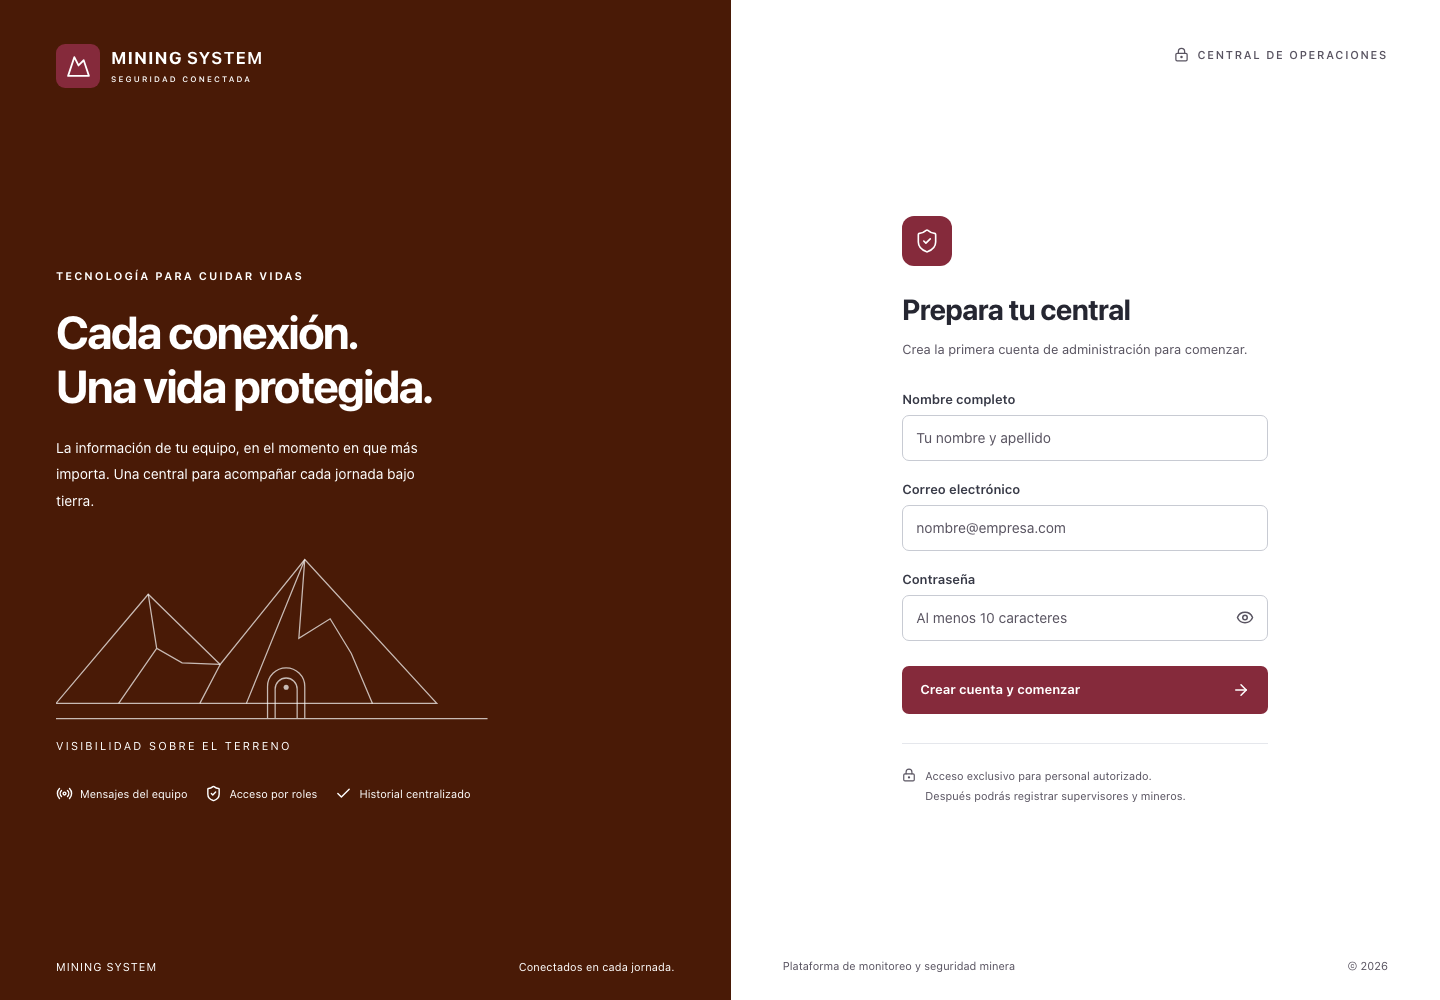
\includegraphics[width=.78\linewidth]{informe/figuras/acceso.png}
\caption{Captura real E-WEB de la pantalla de creación del primer administrador. La prueba comprueba campos obligatorios, correo inválido, longitud mínima y prevención del envío de formularios incompletos.}
\label{fig:acceso}
\end{figure}
\begin{figure}[H]
\centering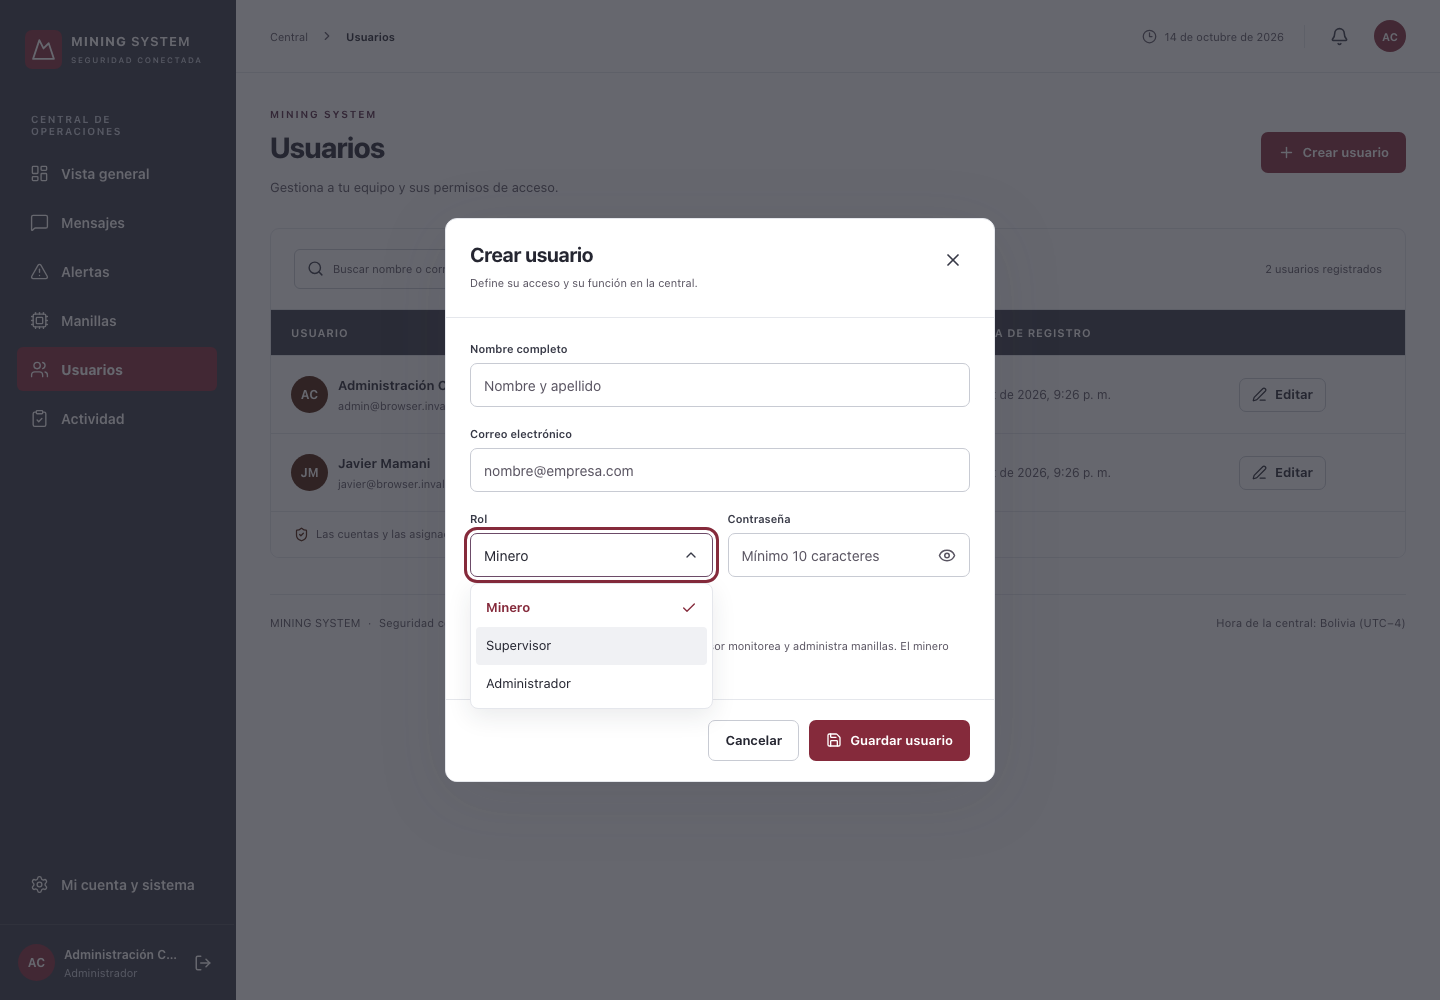
\includegraphics[width=.78\linewidth]{informe/figuras/registro-usuario.png}
\caption{Captura real del formulario de usuarios y selector de roles. Corresponde a un escenario automatizado con cuentas de prueba. Se verifica navegación por teclado, estado activo y comportamiento de los controles.}
\label{fig:registro}
\end{figure}

\newsection{Dashboard y visualización en tiempo real}
\label{sec:dashboard}
\subsection{Implementación real de la interfaz}
El dashboard está desarrollado en \textbf{React 19 y TypeScript}, servido por Vite en desarrollo o Nginx en Docker. Python ejecuta la lógica del nodo; no es el lenguaje del frontend. La interfaz consume la API propia y mantiene una suscripción SignalR para reflejar nuevos registros\cite{signalr}.

La vista general muestra mineros activos, manillas conectadas, mensajes del día y alertas pendientes. También presenta mensajes recientes, cobertura del equipo, distribución por zonas y la última lectura disponible de cada manilla. Mensajes incorpora filtros, búsqueda y exportación de la página actual. Manillas permite consultar el historial de lecturas; Actividad presenta la auditoría administrativa.

\begin{figure}[ht]
\centering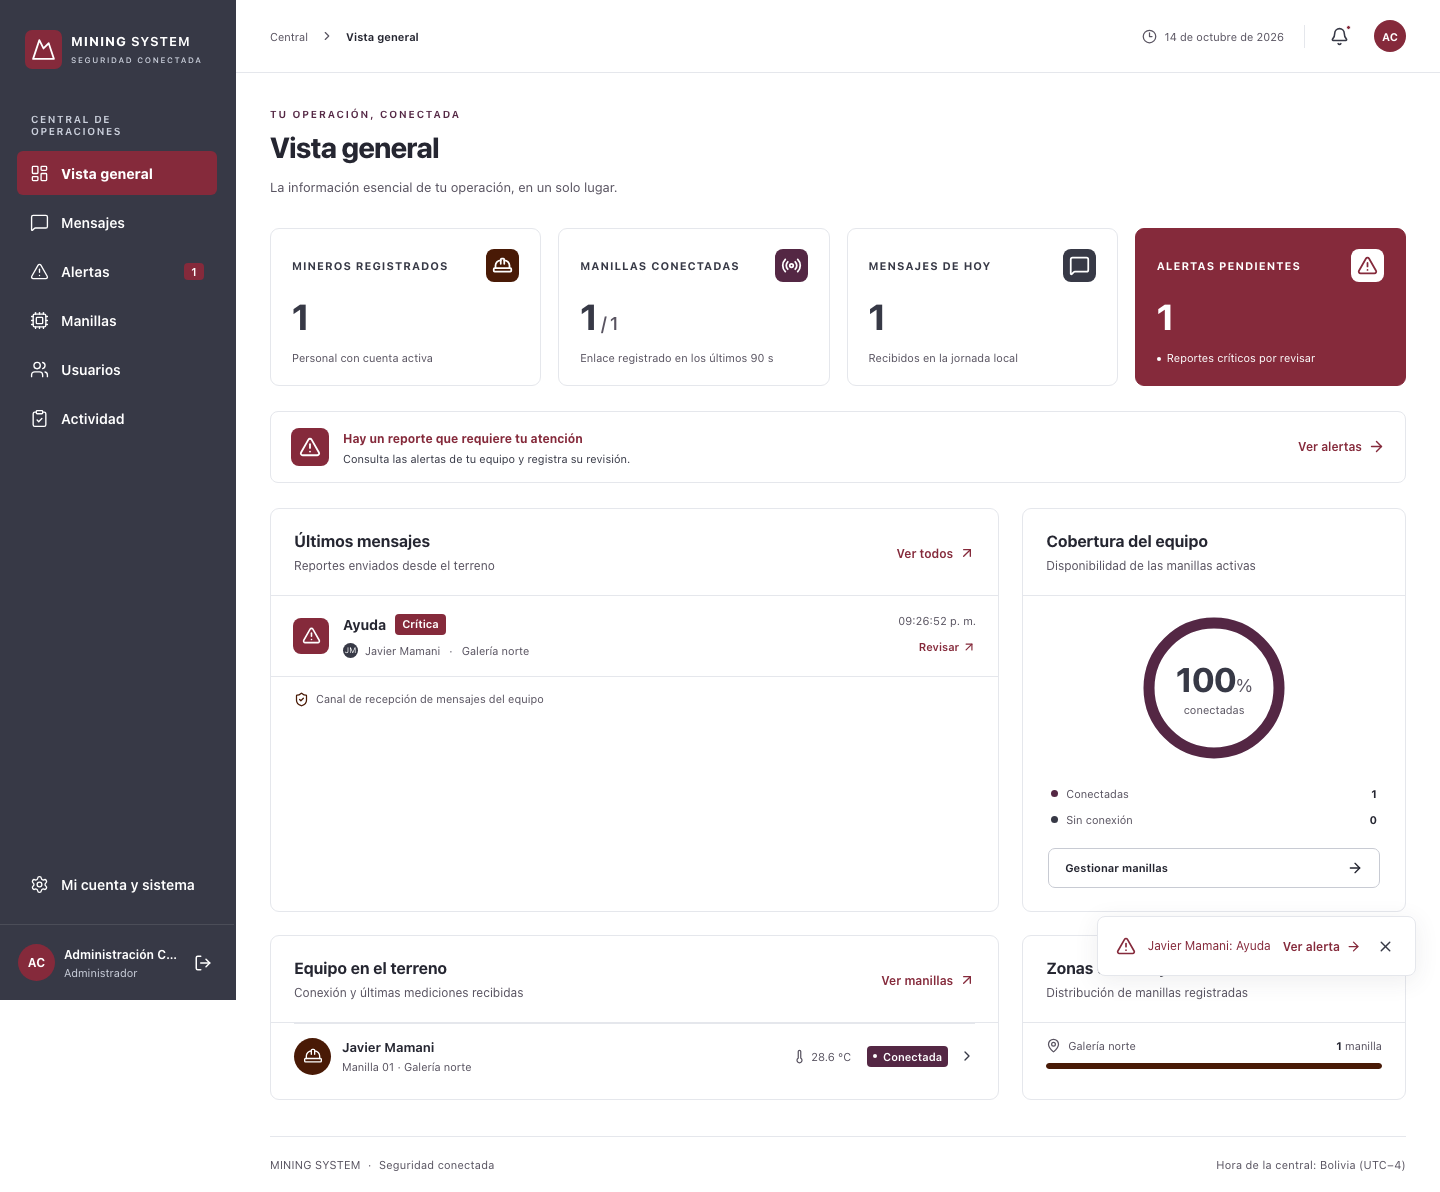
\includegraphics[width=.84\linewidth]{informe/figuras/dashboard.png}
\caption{Dashboard real durante E-WEB con MySQL. Un mensaje de ayuda y una lectura controlada llegan desde el transporte de dispositivo. El 100\,\% visible representa una manilla conectada de una registrada en este escenario, no una métrica de cobertura física de la mina.}
\label{fig:dashboard}
\end{figure}

\subsection{Eventos y recuperación}
\code{MessageReceived} incorpora un reporte persistido; \code{MessageReviewed} actualiza su revisión; \code{TelemetryReceived} notifica una lectura; \code{SystemChanged} comunica cambios de usuarios, dispositivos o presencia. La web vuelve a consultar las vistas necesarias al recibir esos eventos. No se usa sondeo periódico para descubrir mensajes nuevos.

Al reconectar se consultan nuevamente historial y contadores para recuperar eventos ocurridos durante el corte. La interfaz distingue enlace en recuperación, ausencia de red del navegador, presencia del dispositivo y disponibilidad de mediciones. Una manilla desconectada puede conservar una lectura histórica, que no se presenta como medición recién obtenida.

\clearpage
\subsection{Historial, alertas y acceso desde móvil}
\begin{figure}[ht]
\centering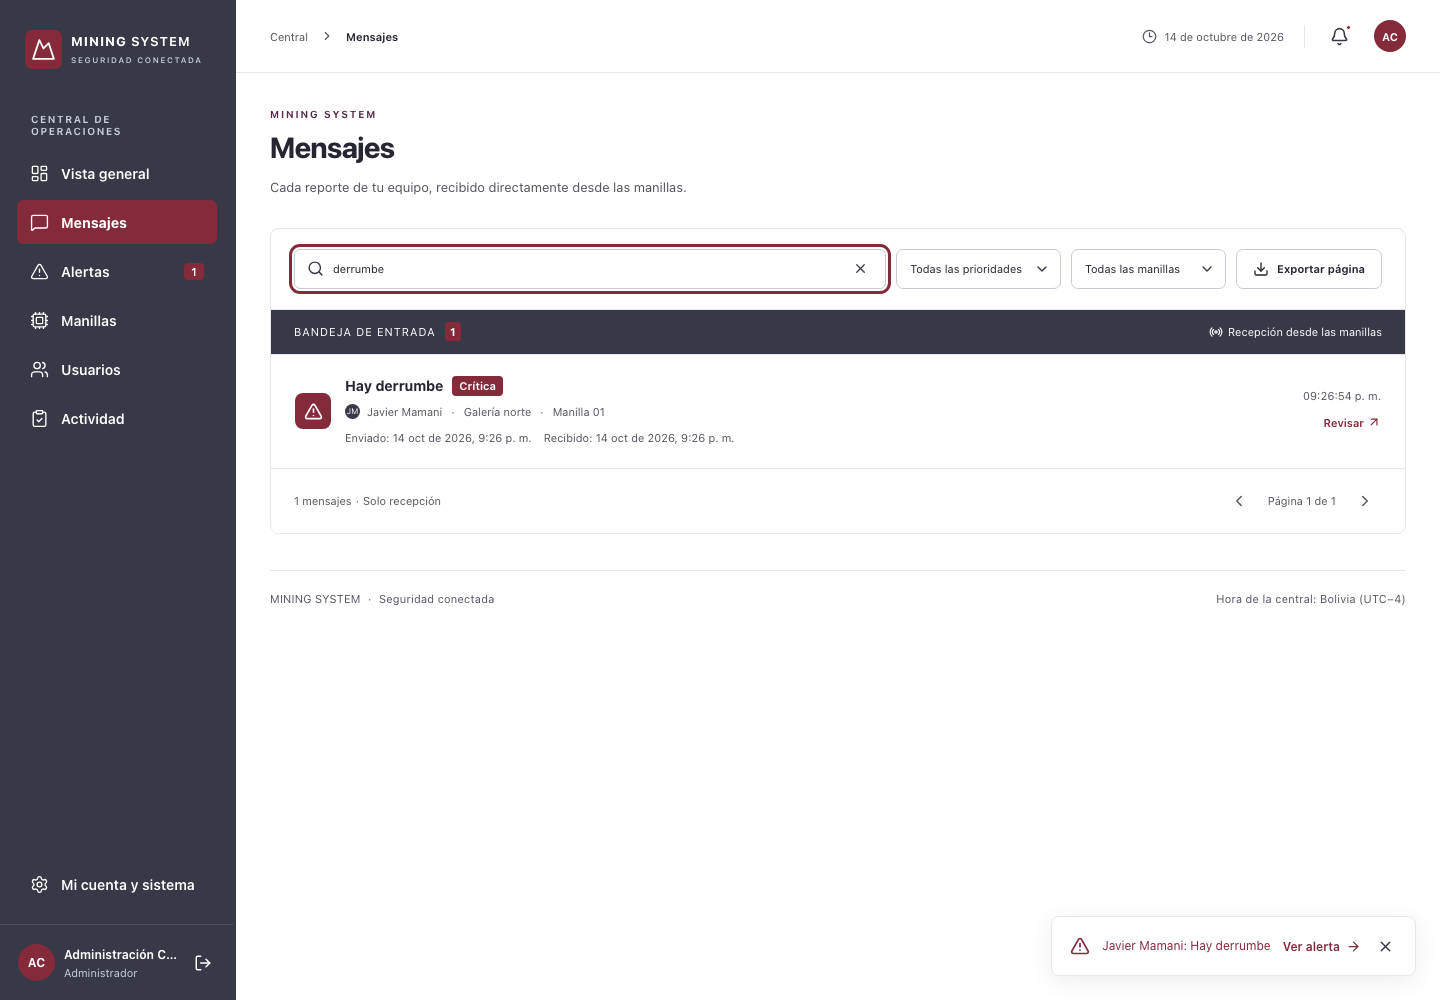
\includegraphics[width=.85\linewidth]{informe/figuras/mensajes.png}
\caption{Historial filtrado por derrumbe en una prueba real de navegador. Se comprueban llegada en vivo, búsqueda y habilitación de la exportación. La revisión de una alerta queda restringida al historial de la central.}
\label{fig:mensajes}
\end{figure}
\begin{minipage}[t]{.58\linewidth}
\subsubsection*{Jerarquía visual y consistencia}
La interfaz utiliza una base clara, navegación lateral y la paleta del proyecto: arena \texttt{\#DEC1AF}, marrón \texttt{\#491A06}, pizarra \texttt{\#373946}, vino \texttt{\#852A3B} y ciruela \texttt{\#6C4B68}. El color destaca prioridad y estado, mientras los textos explican la acción disponible.

Los formularios presentan errores junto a los campos y conservan navegación por teclado. La versión móvil adapta la navegación y el tamaño de los paneles; las pruebas verifican que no aparezca desplazamiento horizontal y que los selectores permanezcan dentro de la pantalla.

\subsubsection*{Límite de la interpretación}
Los reportes críticos proceden de un catálogo explícito. La central no deduce automáticamente un derrumbe ni diagnostica exposición a gas. La telemetría de prueba verifica presentación y persistencia; su lectura física y calibración siguen siendo un trabajo de integración.
\end{minipage}\hfill
\begin{minipage}[t]{.36\linewidth}
\centering\vspace{0pt}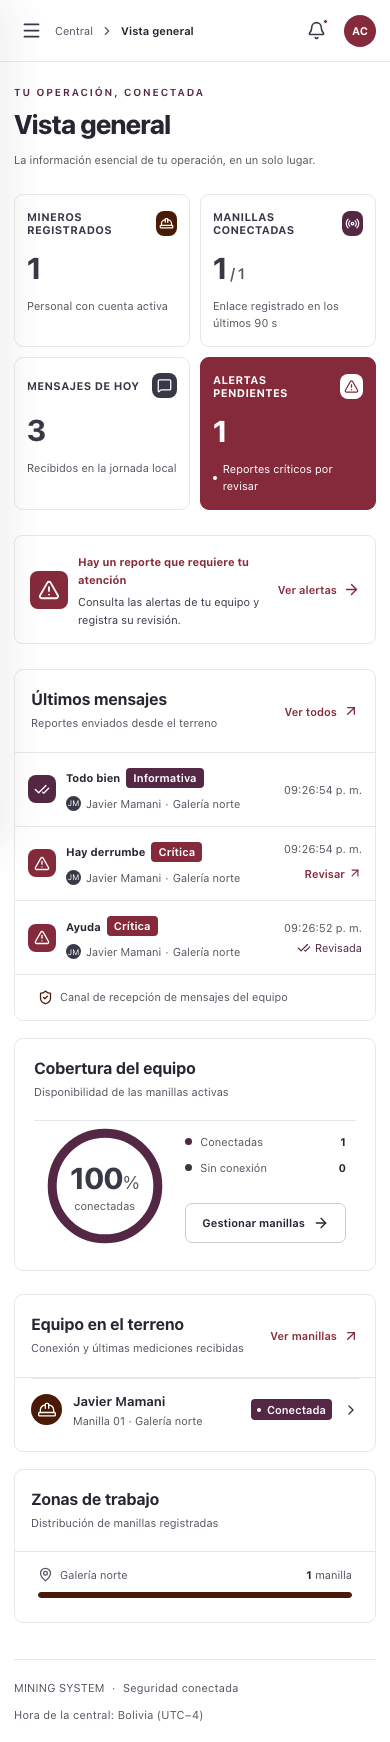
\includegraphics[width=\linewidth,height=96mm,keepaspectratio]{informe/figuras/movil.png}
\captionof{figure}{Captura real de la navegación móvil con un viewport de 390\,$\times$\,844 píxeles.}
\end{minipage}

\newsection{Validación y resultados observados}
\label{sec:validacion}
\subsection{Método y entorno}
Se utilizaron pruebas unitarias de Python, integración contra una API real y MySQL, y escenarios de navegador con Playwright. La integración y el navegador crearon bases temporales independientes de la aplicación y las eliminaron al terminar. Los usuarios y mensajes de demostración no se insertaron en la base migrada del proyecto.

El entorno comprobado utiliza MySQL \code{9.6.0} instalado localmente. Compose define MySQL \code{8.4} LTS para el despliegue. Se validó su configuración, pero no se ejecutó el nuevo stack completo de contenedores en esta sesión porque el daemon de Docker no estaba disponible. Esa comprobación no se contabiliza como una prueba Docker superada.

\begin{tabularx}{\linewidth}{@{}P{27mm}P{24mm}P{22mm}Y@{}}
\toprule\textbf{Nivel} & \textbf{Casos} & \textbf{Resultado} & \textbf{Cobertura relevante}\\\midrule
Dispositivo & 16 & 16 correctos & Menú, GPIO, cola, reinicio, concurrencia y fallos de almacenamiento.\\
API / MySQL & 16 & 16 correctos & Roles, sesión, asignación, WebSockets, lecturas e idempotencia.\\
Navegador & 8 & 8 correctos & Registro, panel, filtros, alertas, reconexión, cuenta y móvil.\\\midrule
\textbf{Total} & \textbf{40} & \textbf{40 correctos} & Ejecuciones reales sobre el software del proyecto.\\\bottomrule
\end{tabularx}

La compilación del backend finalizó sin errores ni advertencias. La compilación de React y el análisis estático pasaron. La configuración Compose y el diagrama Wokwi también se validaron. El total de pruebas aprobadas expresa este conjunto de escenarios; no equivale a cobertura del 100\,\% del código ni a una certificación del hardware.

\subsection{Entrega y persistencia comprobadas}
En E-API se registró una secuencia completa: una consulta anónima fue rechazada, se crearon cuentas y una manilla, se insertó un mensaje, se observó su evento SignalR, se comprobó el reintento y se leyó el historial. MySQL confirmó dos usuarios de prueba, un mensaje y una lectura. El envío duplicado conservó el mismo identificador y no añadió una segunda fila.

Una observación local midió \textbf{\LatenciaLocal\ ms} entre el envío del reporte y la recepción del evento correspondiente en el cliente de SignalR. Se trata de una medición individual dentro del equipo de desarrollo: no es una latencia garantizada, un percentil estadístico ni una prueba de radio en interior mina.

\subsection{Seguridad y continuidad}
Se ensayaron credenciales inválidas y rotadas, roles sin permiso, correos duplicados, protección del último administrador y revocación de sesiones. Otra prueba reinició el servidor y verificó que los registros y las claves de cookie mantuvieran la sesión válida. En el nodo se confirmó que únicamente un ACK coincidente permite retirar un mensaje de la cola.

\clearpage
\subsection{Inventario de evidencias adjuntas}
\begin{longtable}{@{}P{21mm}P{58mm}P{73mm}@{}}
\toprule\textbf{Código} & \textbf{Archivo / origen} & \textbf{Qué demuestra}\\\midrule\endhead
E-CIR & \code{docs/wokwi/diagram.json}; figura~\ref{fig:circuito} & Componentes y conexiones especificadas. Validación estructural con la CLI.\\
E-BD & \code{informe/evidencias/mysql-schema.sql}; figura~\ref{fig:er} & Esquema MySQL generado del modelo EF, relaciones e índices.\\
E-API & \code{informe/evidencias/api-mysql.json} & Diez solicitudes HTTP, respuestas, ACK, duplicado, evento SignalR y conteos consultados en MySQL.\\
E-NODO & \code{informe/evidencias/pruebas-dispositivo.txt}; figura~\ref{fig:oled} & Resultado de 16 pruebas y fotogramas producidos por el software del nodo.\\
E-WEB & \code{informe/figuras/}; \code{web-app/tests/system.spec.ts} & Capturas reales del acceso, registro, dashboard, historial y navegación móvil.\\
E-RES & \code{informe/evidencias/resultados.json} & Resumen de las ejecuciones y límites del entorno verificado.\\
E-LINT & \code{informe/evidencias/lint-web.txt} & Análisis estático del frontend sin incidencias reportadas.\\\bottomrule
\end{longtable}

Los archivos JSON de evidencia ocultan contraseñas y la credencial de la manilla. Las cookies de sesión y los hashes privados no se adjuntan. Las capturas utilizan nombres de demostración y no revelan datos de la cuenta migrada.

\subsection{Cómo reproducir las comprobaciones}
Con MySQL configurado, las herramientas instaladas y desde la raíz:
\begin{lstlisting}[language=bash]
dotnet build backend/backend.csproj
(cd device && .venv/bin/python -m unittest discover -s tests -v)
device/.venv/bin/python -m unittest discover -s tests/backend -v
npm --prefix web-app run build
npm --prefix web-app run lint
(cd web-app && npm run test:e2e)
wokwi-cli lint --offline --warnings-as-errors docs/wokwi
device/.venv/bin/python docs/informe/recolectar.py
\end{lstlisting}
La configuración de pruebas admite variables \code{MINING_TEST_MYSQL_*} o el archivo privado \code{data/mysql-test.json}. El recolector crea su propia base temporal, utiliza datos controlados, registra el intercambio y la elimina al terminar. El usuario de pruebas necesita permisos para crear esas bases; no debe reutilizarse una base de producción como escenario de ensayo.

\newsection{Despliegue, operación y continuidad}
\label{sec:despliegue}
\subsection{Central con tres servicios}
\code{compose.yaml} define MySQL, el backend y la web con Nginx. Solo el proxy publica el puerto HTTP; MySQL permanece en la red privada. El backend espera a que el motor esté saludable, aplica las migraciones y conserva fuera de las imágenes las claves de protección de sesión. Los volúmenes separan los datos del motor y los datos operativos del servidor.

\code{start.sh} genera contraseñas aleatorias cuando faltan, compila las imágenes, inicia los servicios y espera su estado de salud. Las credenciales se montan mediante secretos y no se incluyen en el repositorio. La cuenta de la API tiene permisos sobre la base del proyecto; la contraseña de administración se mantiene aparte.

\begin{lstlisting}[language=bash]
./start.sh                    # Compilar e iniciar
docker compose ps             # Revisar el estado
docker compose logs --tail=100 # Consultar registros
./start.sh --down              # Detener y conservar volumenes
\end{lstlisting}

El nombre previsto de la central es \code{franco-rasp4.local}. Nginx redirige \code{/api}, \code{/hubs/mining} y \code{/ws/device}, manteniendo un origen único y el cambio de protocolo para WebSocket. La resolución mDNS depende de la red y del servicio del sistema; el programa no cambia el hostname.

\subsection{Respaldo y evolución}
Un respaldo consistente incluye un volcado lógico de MySQL, las claves de sesión y los secretos de conexión. \code{mysqldump --single-transaction --no-tablespaces} permite respaldar las tablas del proyecto con la cuenta correspondiente. Los respaldos contienen información de usuarios y hashes, por lo que se mantienen privados y fuera de Git.

El esquema se evoluciona con migraciones versionadas. El procedimiento \code{--import-legacy} es una herramienta puntual para trasladar datos anteriores a una base vacía, no un mecanismo para mezclar dos instalaciones. Borrar volúmenes no forma parte del ciclo normal de actualización.

\subsection{Puesta en marcha del nodo}
En Raspberry Pi OS se habilitan I\textsuperscript{2}C y el overlay de I\textsuperscript{2}S especificado en la guía de conexiones. Se instala el entorno virtual de Python, se configura la URL de la central y se copia la credencial de la manilla. El directorio de cola se conserva entre reinicios. El arranque puede automatizarse con el servicio systemd documentado.

El uso de HTTPS/WSS, la cobertura de radio real, la autonomía, el encapsulado, la calibración y la validación de sensores requieren comprobación en el entorno de despliegue. No se presentan como resultados ya medidos en este informe.

\newsection{Correspondencia con la evaluación y defensa}
\label{sec:evaluacion}
\subsection{Cobertura de los temas solicitados}
La evaluación suma 100 puntos. La tabla relaciona cada tema con la evidencia de esta implementación; no asigna una calificación ni sustituye la revisión del docente.

\begin{tabularx}{\linewidth}{@{}P{42mm}P{13mm}Y@{}}
\toprule\textbf{Tema de evaluación} & \textbf{Peso} & \textbf{Desarrollo documentado}\\\midrule
Diseño del circuito IoT & 10 & Componentes, alimentación, buses, mapa BCM/físico, protección del motor y plano. Sección~\ref{sec:circuito}.\\
Base de datos y diagrama & 5 & Modelo MySQL, ER, integridad, índices, migraciones y esquema SQL. Sección~\ref{sec:datos}.\\
Integración REST, inserción y lectura & 15 & API propia para gestión/consulta; ingestión WebSocket y persistencia real MySQL. No se usa Supabase. Sección~\ref{sec:api}.\\
Programa del nodo & 15 & Python 3 sobre Linux, interfaz y envío persistente. Esta plataforma usa CPython, no MicroPython. Sección~\ref{sec:python}.\\
Registro y autenticación & 15 & Alta inicial, administración de cuentas, hash, cookie, roles y revocación. Sección~\ref{sec:auth}.\\
Dashboard en tiempo real & 15 & Dashboard implementado en React/TypeScript con SignalR; Python corresponde al nodo. Sección~\ref{sec:dashboard}.\\
Informe, exposición y defensa & 25 & Memoria técnica, pruebas, límites, anexos y guion de demostración. Secciones~\ref{sec:validacion}--\ref{sec:evaluacion}.\\\bottomrule
\end{tabularx}

\subsection{Guion de exposición sugerido}
\begin{enumerate}
\item \textbf{Problema y arquitectura (2 minutos):} identificar trabajador, nodo, central y recorrido del mensaje; mostrar la figura~\ref{fig:arquitectura}.
\item \textbf{Circuito y datos (3 minutos):} explicar I\textsuperscript{2}C compartido, entrada analógica, transistor del motor, relaciones MySQL e idempotencia.
\item \textbf{Demostración funcional (4 minutos):} iniciar sesión, registrar un minero/manilla, emitir un reporte de prueba, observar su llegada y revisar la alerta. Indicar cuándo se está usando el simulador.
\item \textbf{Continuidad y seguridad (2 minutos):} explicar la cola, un reintento y la separación entre roles y credenciales de dispositivo.
\item \textbf{Resultados y límites (1 minuto):} resumir las 40 pruebas y el estado pendiente de sensores, calibración y campo.
\end{enumerate}

\clearpage
\subsection{Preguntas técnicas que deben poder defenderse}
\begin{description}[style=nextline,leftmargin=0pt,labelwidth=0pt,labelsep=0pt,font=\bfseries\color{Wine}]
\item[¿Por qué se necesita el ADS1115?] El SEN0564 entrega una salida analógica y la Pi no ofrece un ADC integrado. El conversor digitaliza A0 y comparte I\textsuperscript{2}C con direcciones diferentes.
\item[¿Qué garantiza que un mensaje no se pierda al cortar la red?] Antes de enviarlo se persiste en la cola local. Se conserva hasta un ACK coincidente; al recuperar el enlace se reintenta con el mismo identificador.
\item[¿Por qué no aparecen duplicados al perder una confirmación?] MySQL impone unicidad sobre dispositivo e identificador de origen. El servidor reconoce el registro existente y devuelve el mismo ID.
\item[¿Por qué MySQL y por qué una cola local diferente?] MySQL centraliza las entidades relacionales. La cola es un mecanismo de transporte que debe seguir escribiendo cuando la central está inaccesible; por eso reside en archivos locales de la manilla.
\item[¿Cuál es la diferencia entre REST y WebSocket en este proyecto?] REST atiende solicitudes de gestión y consulta. WebSocket transporta eventos del nodo, y SignalR actualiza la interfaz a partir de registros persistidos.
\item[¿Qué significa el estado Enviado a central?] Que el servidor confirmó persistencia. No significa que un supervisor haya leído el reporte ni que el incidente esté resuelto.
\item[¿Los 410 ppm de las pruebas demuestran medición de CO?] No. Son un dato controlado para verificar el transporte y la visualización. Una lectura real en ppm exige integrar y calibrar el sensor.
\item[¿Se utilizó MicroPython o un dashboard Python?] No. El nodo usa CPython sobre Raspberry Pi OS; el panel usa React y TypeScript. Se pueden explicar esas decisiones sin atribuir herramientas que el sistema no utiliza.
\end{description}

\section{Conclusiones}
\label{sec:conclusiones}
El proyecto demuestra un flujo verificable de comunicación desde la interfaz del nodo hasta un historial centralizado y un panel actualizado por eventos. La confirmación explícita, el identificador estable y la persistencia local separan la intención de enviar de la entrega efectivamente confirmada.

La migración a MySQL mantiene el modelo del dominio y los datos existentes, introduce un esquema versionado y conserva los contratos de la API y la interfaz. Las pruebas de integración y navegador verificaron que autenticación, registro, mensajes, lecturas y recuperación continúan funcionando con el nuevo motor.

Los principales resultados comprobados son las 40 pruebas satisfactorias, la inserción y lectura reales en MySQL, la idempotencia de mensajes y la propagación SignalR. El siguiente trabajo técnico consiste en integrar y calibrar sensores y actuadores, comprobar autonomía y cobertura, y validar el conjunto físico antes de atribuirle funciones de seguridad en campo.

\clearpage
\begin{thebibliography}{12}
\small
\bibitem{rpi} Raspberry Pi. \emph{Raspberry Pi Zero 2 W: especificaciones oficiales}. \url{https://www.raspberrypi.com/products/raspberry-pi-zero-2-w/}.
\bibitem{co} DFRobot. \emph{Fermion MEMS CO Sensor, SEN0564}. \url{https://wiki.dfrobot.com/sen0564/}.
\bibitem{mysql} Oracle MySQL. \emph{Connector/NET: Entity Framework Core}. \url{https://dev.mysql.com/doc/connector-net/en/connector-net-entityframework-core.html}.
\bibitem{provider} Oracle MySQL. \emph{MySql.EntityFrameworkCore 10.0.9}. \url{https://www.nuget.org/packages/MySql.EntityFrameworkCore/10.0.9}.
\bibitem{cookie} Microsoft. \emph{Cookie authentication in ASP.NET Core}. \url{https://learn.microsoft.com/en-us/aspnet/core/security/authentication/cookie?view=aspnetcore-10.0}.
\bibitem{signalr} Microsoft. \emph{Overview of ASP.NET Core SignalR}. \url{https://learn.microsoft.com/en-us/aspnet/core/signalr/introduction?view=aspnetcore-10.0}.
\bibitem{wokwi} Wokwi. \emph{Formato de diagram.json y Wokwi CLI}. \url{https://docs.wokwi.com/diagram-format}.
\bibitem{elements} Wokwi. \emph{Wokwi Elements, versión 1.9.2; licencia MIT}. \url{https://github.com/wokwi/wokwi-elements}.
\bibitem{proyecto} Franco Parra. \emph{Mining System: código y documentación del proyecto}. Repositorio local: \code{backend/}, \code{device/}, \code{web-app/}, \code{tests/} y \code{docs/}. Versión examinada el 14 de octubre de 2026, con migración MySQL validada en esa fecha local.
\end{thebibliography}

\appendix
\newsection{Evidencia ejecutable y organización de la entrega}
La entrega incluye el fuente \code{informe_final.tex}, las figuras, los archivos de evidencia y el PDF compilado. Los elementos generados se agrupan bajo \code{docs/informe/}. La ilustración del circuito mantiene sus créditos en \code{docs/wokwi/assets/}.

\begin{lstlisting}
docs/
  informe_final.tex
  informe_final.pdf
  mysql-schema.sql
  mysql.md
  informe/
    datos.tex
    recolectar.py
    figuras/       # Capturas reales, OLED y circuito
    evidencias/    # API/MySQL, esquema y resultados
\end{lstlisting}

\subsection*{Compilar el informe}
\begin{lstlisting}[language=bash]
cd docs
latexmk -xelatex -interaction=nonstopmode -halt-on-error informe_final.tex
\end{lstlisting}
Se utiliza una fuente incluida en TeX Live, sin depender de tipografías de pago ni de archivos de una cuenta externa. Las imágenes se resuelven mediante rutas relativas.

\subsection*{Fragmento del contrato de almacenamiento MySQL}
El siguiente extracto procede del esquema generado por EF Core, no de una tabla propuesta sin implementar. El archivo adjunto conserva las cinco entidades e índices completos.
\lstinputlisting[language=SQL,firstline=1,lastline=16]{informe/evidencias/mysql-schema.sql}

\subsection*{Prueba documental de datos controlados}
\lstinputlisting[language=JSON]{informe/evidencias/resultado-resumen.json}

\end{document}
